\chapter{Methodology}

This project has a predominantly quantitative computing and \gls{gis}-based methodology, which includes the use of \glspl{api} for automated data downloads, geostatistics and geovisualisation, exploratory data analysis, raster and vector data processing, viewshed analysis, and \gls{mca}. To supplement this data, qualitative inputs are obtained through a participatory \gls{gis} session with community land owners.

The data used in this project are predominantly derived from a number of UK or Scottish public sector data sources, including Ordnance Survey, Scottish Government, Marine Scotland, NatureScot, Improvement Service, and Historic Environment Scotland \autocite{os-downloads,spatialdata}. Additionally, bathymetry data used is derived from the European Union's EMODnet Bathymetry portal \autocite{emodnet-bathymetry}. All downloaded data are in the EPSG:27700 (Ordnance Survey National Grid reference system); except for data downloaded from Marine Scotland and EMODnet, which are in EPSG:4326. The output data produced are in the EPSG:27700 \gls{crs} and two file formats: GeoPackage for vector data (points, lines, and polygons), and GeoTIFF for raster data.

This project uses a number of open-source software packages and dependencies, including the QGIS Geographic Information System, GDAL/OGR Geospatial Data Abstraction software Library, and the Python Programming Language and its geospatial libraries, including GeoPandas \autocite{qgis,gdal,python,geopandas}. The analysis can be performed cross-platform on a personal computer with 64-bit processing architecture.

The overall methodology used is summarised in the flowcharts in \autoref{fig:flowcharts}. A full list of data and software used, as well as a link to view the Python scripts, can be found in \autoref{app:data} and \autoref{app:soft}.

\begin{figure}
  \centering
  \begin{subfigure}[t]{.96\textwidth}
    \centering
    \includegraphics[scale=.6]{../images/flowchart1}
  \end{subfigure}
  \\
  \begin{subfigure}[t]{.96\textwidth}
    \centering
    \includegraphics[scale=.6]{../images/flowchart2}
  \end{subfigure}
  \caption{Flowcharts summarising the computational and GIS methodologies used. \label{fig:flowcharts}}
\end{figure}

\section{Study area}

The \gls{smp} Plan Option polygons were downloaded from Marine Scotland. Using the GeoPandas Python library, the dataset was filtered to include only site N4, and then reprojected into EPSG:27700. The resulting polygon was opened using the QGIS user interface, with Ordnance Survey's 1:250 000 Scale Colour Raster for the Isle of Lewis area, comprising of the NA, NB, and NG British National Grid 100 km tiles added as a basemap for context.

A study area around site N4 is determined to confine the analysis to a limited area, which enables the analysis to focus on the impacts on the communities closest to the shore, as well as improve the computational efficiency of the analysis by using a subset of all data available. An initial enquiry on the profiles of the land owners interested in taking part in this project was done to find their locations of interest. These locations were found on the basemap to be within a 15 km buffer from the edges of site N4; as a result, the area occupied by this buffer is selected as the final study area. The buffer was created and saved as a polygon using Python.

In order to provide additional context to the study area, boundaries representing community councils, which are statutory bodies independently run by volunteer residents representing communities \autocite{cnes-cc}, were used. These were downloaded, along with the Ordnance Survey Boundary-Line\texttrademark\ administrative boundary data, using a Python script, with the 15 km buffer serving as a mask to clip the data to the study area.

A map showing these community councils within the study area can be seen in \autoref{fig:cc-study}. Based on the map, eight community council areas are affected: Airidhantuim, Barvas and Brue, Bernera, Breasclete, Carloway, Ness, Shawbost, and Uig. It can be observed that the overlayed community council polygons do snap some areas, particularly the small islands close to Bernera and Uig, which was also noted in the data download source. As a result, if these polygons are used to cluster points, some data points will be out of bounds. This will be rectified in the sections below.

\begin{figure}
  \centering
  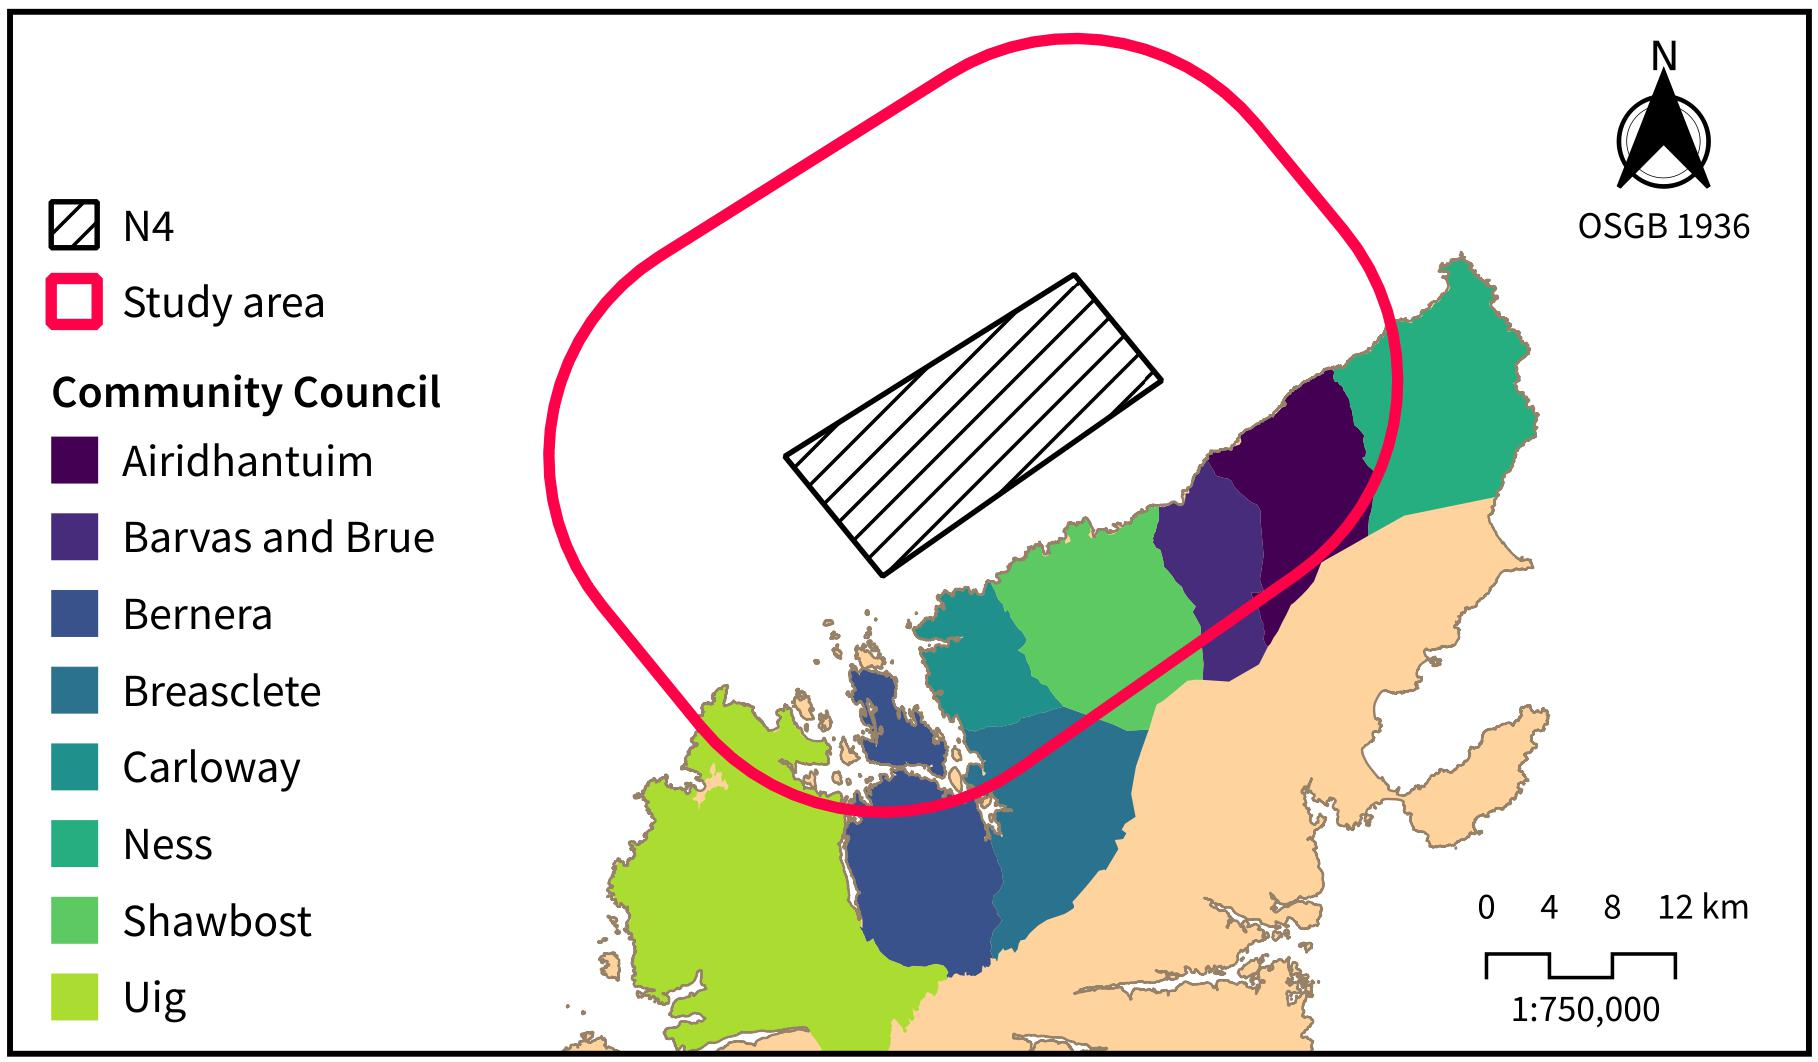
\includegraphics{../images/maps/study_area}
  \caption{A map showing the location of Sectoral Marine Plan option N4 and the study area boundary relative to community council areas in the Isle of Lewis. \label{fig:cc-study}}
\end{figure}

\newpage
\subsection{Digital terrain model}

A \gls{dtm} for the study area was then generated. A number of data sources were consulted, including high-resolution (50 cm to 2 m) LiDAR elevation models by the Scottish Environment Protection Agency \autocite{sepa-lidar}. However, once merged, the \gls{dtm} was 12 GB large and did not include part of the study area near Bernera and Uig. Ordnance Survey's OS Terrain\textregistered\ 50 dataset includes 10 m contour lines together with a number of spot heights, which can be interpolated to generate a much smaller \gls{dtm} of 10 m resolution. However, this only covers the land area. Bathymetry data covering the study area was not available; as a result, the EMODnet Digital Bathymetry \gls{dtm} in ASCII raster format was used. The bathymetry data had a resolution of 81 m and the EPSG:4326 \gls{crs}.

To derive elevation data from the bathymetry layer for the interpolation, the raster was first converted into points using QGIS's raster pixels to points algorithm. Then, the points were reprojected into EPSG:27700. After clipping the elevation datasets to the study area, a 10 m \gls{dtm} (pixel size of 10) was generated using QGIS's triangulated irregular network (TIN) interpolation algorithm. The resulting \gls{dtm} can be seen in \autoref{fig:dtm}.

\begin{figure}
  \centering
  \includegraphics{../images/maps/hillshade_dtm}
  \caption{A map showing the digital terrain model of the study area. \label{fig:dtm}}
\end{figure}

\section{Visual impact assessment}

\subsection{Scenario development}

To assess the visual impacts of offshore wind turbines on the island communities, a number of scenarios representing wind farm development alternatives were constructed. Since there have not been any applications by developers to construct a wind farm at site N4 thus far, there is possibility to explore a large number of scenarios. To limit this, a number of constraints were first defined. This project's focus is on the impacts of development at site N4 on communities. Therefore, the site's suitability in terms of electricity grid connectivity, geology, meteorology, atmospheric conditions, etc. are deemed out of scope of the project.

The technological trends and learning curves, as well as downwind and crosswind spacing are also not within the scope of this project; approximate turbine specifications are used in line with recently established offshore wind farms in Scotland. A list of offshore wind farm projects in Scotland, both operational and under construction, are shown in \autoref{tab:offshore}. This table includes information about the capacity of turbines used, the height of these turbines, and the minimum spacing between turbines, compiled from publicly available development specification and layout plans available on Marine Scotland \autocite{ukgov-repd,beatrice,nng-wind,moray-east,inchcape,moray-west,seagreen}. The heights are measured to the tip of the turbine from either the lowest or highest astronomical tide, or both, depending on the specification document. The lowest astronomical tide measurements were around 5 m more than the highest astronomical tide measurements.

\begin{longtable}{lrrr}
  \caption{List of offshore wind projects in Scotland in the last decade, compiled using development specification and layout plans available on Marine Scotland. \label{tab:offshore}} \\

  \toprule
  \multicolumn{1}{l}{\textbf{Name}} &
  \multicolumn{1}{l}{\textbf{Turbine capacity (MW)}} &
  \multicolumn{1}{l}{\textbf{Turbine height (m)}} &
  \multicolumn{1}{l}{\textbf{Turbine spacing (m)}} \\
  \midrule
  \endfirsthead

  \multicolumn{4}{c}
  {{\textbf{\tablename\ \thetable{}} -- continued from previous page}} \\
  \toprule
  \multicolumn{1}{l}{\textbf{Name}} &
  \multicolumn{1}{l}{\textbf{Turbine capacity (MW)}} &
  \multicolumn{1}{l}{\textbf{Turbine height (m)}} &
  \multicolumn{1}{l}{\textbf{Turbine spacing (m)}} \\
  \midrule
  \endhead

  \midrule
  \multicolumn{4}{r}{{Continued on next page}} \\
  \bottomrule
  \endfoot

  \endlastfoot

  Beatrice & 7.000 & 187.0 & 945.5 \\
  Neart na Gaoithe & 8.000 & 208.0 & 907.0 \\
  Moray East & 9.525 & 198.9 & 1,128.0 \\
  Seagreen & 10.000 & 205.0 & 1,042.0 \\
  Moray West & 10.000 & 230.0 & 1,050.0 \\
  Inch Cape & 15.000 & 291.0 & 1,278.0 \\

  \bottomrule
\end{longtable}

Based on this table, offshore turbines up to 291 m and 15 MW are being erected in Scottish waters, with no turbine less than 187 m and 7 MW in the last decade. The spacing between turbines tend to increase with increasing turbine heights and rated power (which also means larger blades and rotor diameters). However, while the spacing is generally in the order of a 1,000 m, there is no clear correlation of the spacing with the height and capacity of the turbine. The spacing is additionally influenced by the total area available for the wind farm development.

The specification and layout plans also detail the water depths below the lowest astronomical tide at the development site, which ranged from 38-59 m. To gain a general understanding of the seabed's condition at site N4, a histogram showing the depth distribution of the area was obtained using the \gls{dtm}'s pixel values, which is shown in \autoref{fig:hist}. With a mean depth of 53 m and the entire range within three standard deviations, site N4's depth profile is similar to that of the other offshore wind farm projects.

\begin{figure}
  \centering
  \frame{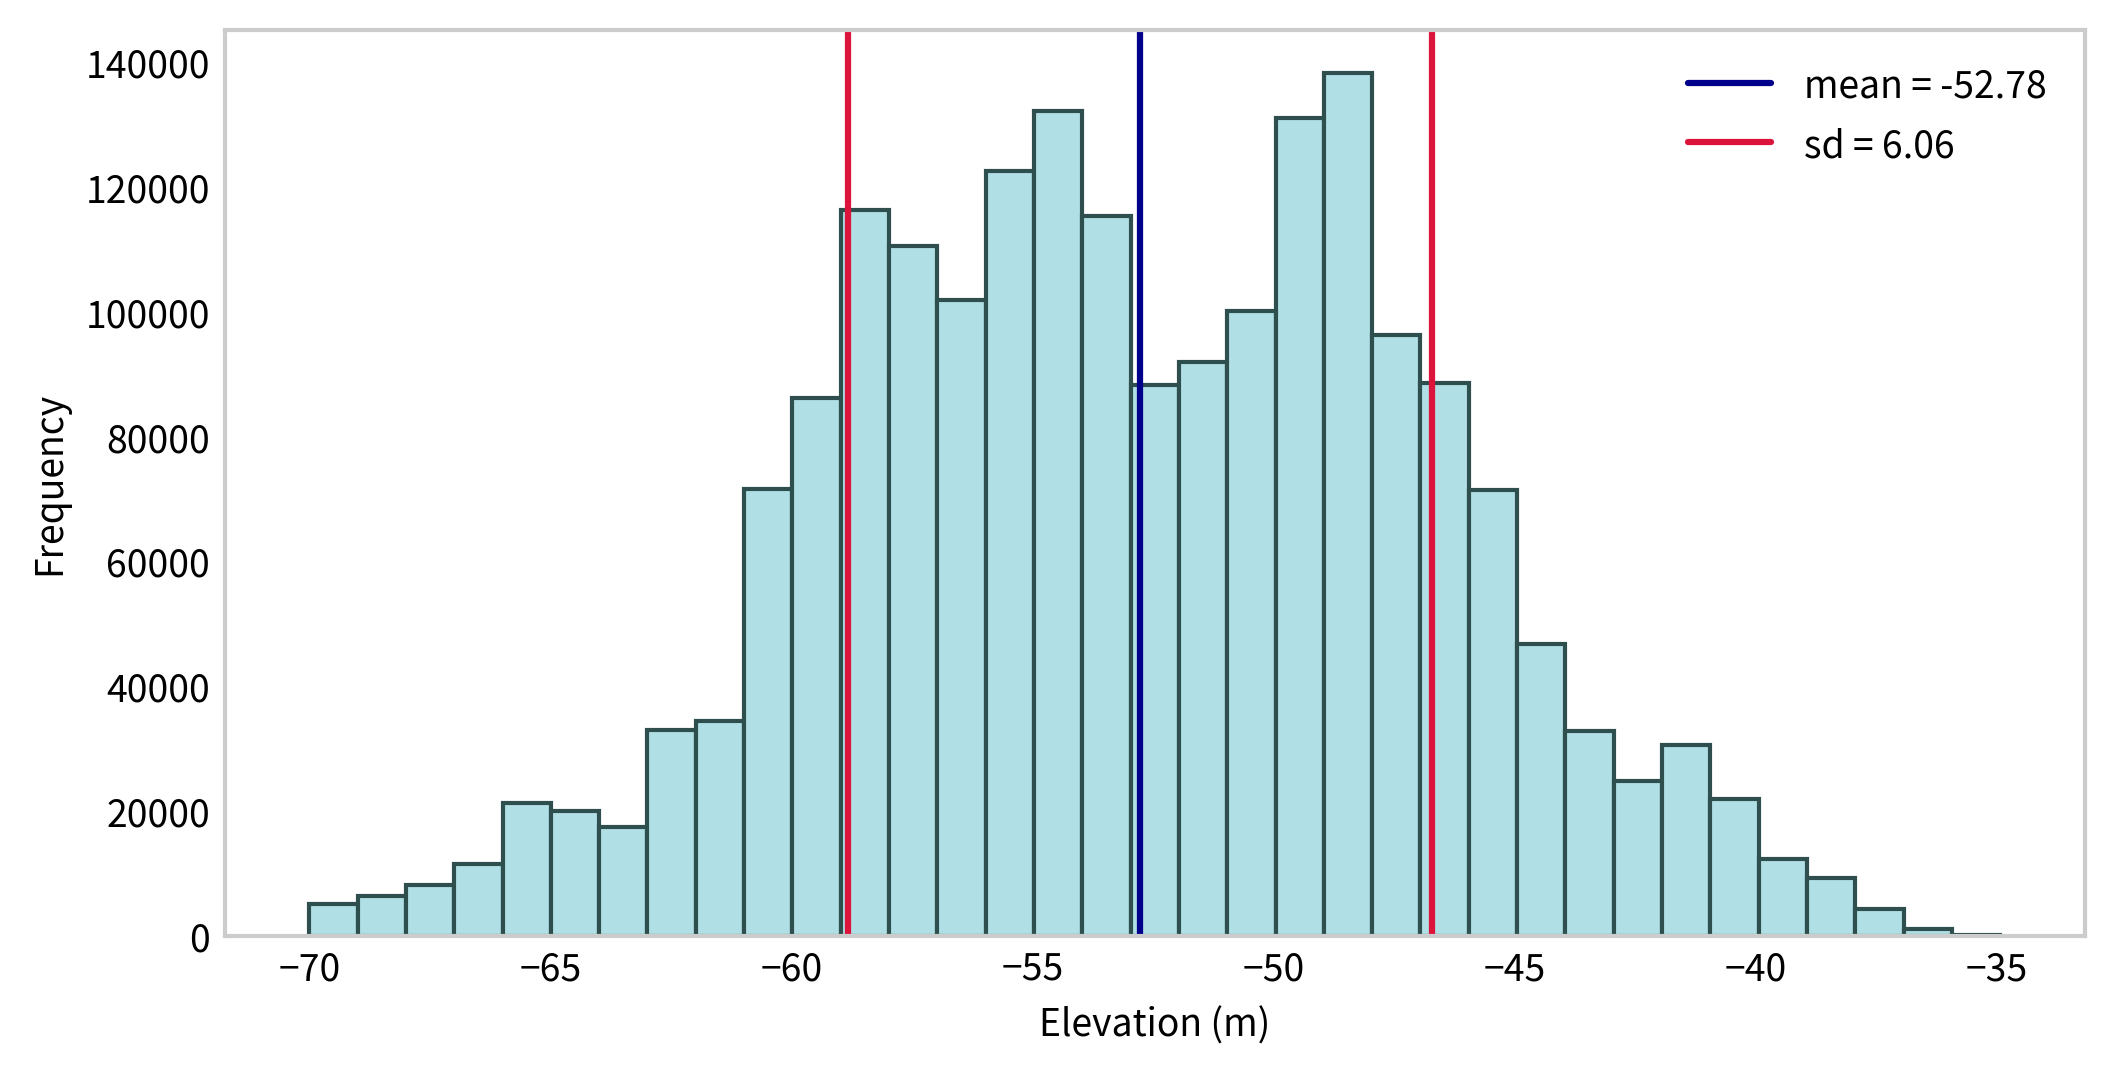
\includegraphics[width=.9\textwidth]{../images/plots/histogram}}
  \caption{A histogram showing the distribution of water depth within site N4. \label{fig:hist}}
\end{figure}

Once the draft \gls{smp} was released in December 2019, NatureScot published a response to their consultation with a design guidance for each Plan Option \autocite{naturescot-smp}. In this document, they recommend wind turbines of heights less than 200 m to mitigate the significant changes to the landscape and seascape of the Isle of Lewis. Therefore, in this analysis, the maximum turbine height considered is 200 m, with an estimated power rating of 10 MW based on similar turbines in \autoref{tab:offshore}. Two additional heights are considered: 180 m (8 MW) and 160 m (6 MW). By keeping the number of turbines constant, the effects of turbine height on visual impacts can be quantified. A fixed number of 25 turbines are used for this analysis.

Additionally, scenarios with varying number of turbines are also used to simulate the visual impacts based on turbine density. A constant height of 180 m is used for these turbines, and the number of turbines used are 100, 75, 50, and 25. A summary of these scenarios is shown in \autoref{tab:scenarios}. This gives a total of six unique scenarios, where four are used to compare the effects of varying turbine numbers, and three are used to compare the effects of varying turbine heights.

\begin{longtable}{rrrr}
  \caption{List of scenarios to simulate different number of wind turbines at various heights and installed capacities. \label{tab:scenarios}} \\

  \toprule
  \multicolumn{1}{l}{\textbf{Number of turbines}} &
  \multicolumn{1}{l}{\textbf{Turbine height}} &
  \multicolumn{1}{l}{\textbf{Turbine capacity (MW)}} &
  \multicolumn{1}{l}{\textbf{Wind farm capacity (MW)}} \\
  \midrule
  \endfirsthead

  \multicolumn{4}{c}
  {{\textbf{\tablename\ \thetable{}} -- continued from previous page}} \\
  \toprule
  \multicolumn{1}{l}{\textbf{Number of turbines}} &
  \multicolumn{1}{l}{\textbf{Turbine height}} &
  \multicolumn{1}{l}{\textbf{Turbine capacity (MW)}} &
  \multicolumn{1}{l}{\textbf{Wind farm capacity (MW)}} \\
  \midrule
  \endhead

  \midrule
  \multicolumn{4}{r}{{Continued on next page}} \\
  \bottomrule
  \endfoot

  \endlastfoot

  100 & 180 & 8 & 800 \\
  75 & 180 & 8 & 600 \\
  50 & 180 & 8 & 400 \\
  25 & 200 & 10 & 250 \\
  25 & 180 & 8 & 200 \\
  25 & 160 & 6 & 150 \\

  \bottomrule
\end{longtable}

For these scenarios to be used as geographical inputs for viewshed analysis, they must first be converted into points. It is assumed that the turbines are distributed in an array of equidistant points. During the actual project planning phase of an offshore wind farms, there will be additional constraints to consider when determining wind turbine placement, such as geological formations, wave conditions, and underwater cabling, which are all out of scope of this research project. There is no straightforward way to generate a certain number of equidistant points inside a polygon. With some trial and error using QGIS's regular points and intersection algorithms, points representing turbines at equal distance were generated. The distances are:

\begin{itemize}[noitemsep]
  \item 2,880 m for 25 turbines,
  \item 2,000 m for 50 turbines,
  \item 1,625 m for 75 turbines, and
  \item 1,400 m for 100 turbines.
\end{itemize}

All distances are above the 1,000 m range deduced from \autoref{tab:offshore}. The spatial distribution of these points within site N4 can be viewed in \autoref{fig:turbine-number}.

\begin{figure}
  \centering
  \includegraphics{../images/maps/scenarios}
  \caption{Maps demonstrating the offshore wind development scenarios in terms of number of wind turbines which are distributed equally within site N4. \label{fig:turbine-number}}
\end{figure}

\newpage
\subsection{Viewshed analysis}

After the scenarios were developed, a binary viewshed analysis was conducted. This was done using GDAL's viewshed algorithm, which comes preinstalled with QGIS. A number of parameters are defined in this algorithm. The input raster provided is the \gls{dtm} generated earlier. The observer locations are the wind turbine points. The observer height is the height of the turbine, plus 50 m to take into account the displacement between the seabed and the water surface. Finally, a visibility distance must be provided.

NatureScot's guidance on visual representation of wind farms \autocite{naturescot-visual} recommends a distance of 45 km or more for wind turbines taller than 150 m and all offshore wind turbines in general, for performing \gls{ztv} calculations. This distance will cover the entirety of the study area, as it is confined to a 15 km buffer around the borders of the N4 site. A target height of 1.65 m was provided to represent a 1.65 m tall human on the terrain model.

This GDAL algorithm only accepts one observer point per run. Therefore, a Python script, which iterates across each point in the turbine array layer was written. This results in one binary viewshed output (GeoTIFF raster) being produced for each turbine.

To generate a cumulative raster for each scenario, QGIS's raster calculator to add all of the raster layers together. The results were then clipped to the land area using GDAL's clip raster by mask layer algorithm. The resulting raster files will have a continuous scale. To obtain discrete scales, showing areas with negligible, slight, moderate, substantial, and severe visual impacts (as suggested in \cite{falconer2013}), each cumulative raster was reclassified using five discrete classes with values between 0 and 1, where 1 represents severe impact and 0 represents negligible impact.

\subsection{Viewpoints}

To evaluate the visual impacts on specific viewpoints in the study area, cultural heritage data from Historic Environment Scotland was consulted. Scheduled monuments are monuments classed as being important nationally; designations are done by Historical Environment Scotland under Ancient Monuments and Archaeological Areas Act 1979, as well as the Designation Policy and Selection Guidance \autocite{hes-scheduling}.

The data was first downloaded from Historic Environment Scotland's \gls{api} using Python. Using the study area buffer polygon, the data was clipped to the study area. To cluster the monuments into their respective community councils, a spatial join was performed using GeoPandas between the two dataframes, keeping the geometry attributes of the scheduled monuments data. When tested, it was found that two entries, namely Beinn an Teampuill, Little Bernera and St Peter's Church, Pabay Mor, were not assigned a community council area due to the gaps present in the community council boundary data. By cross-referencing these points with Canmore data \autocite{canmore}, they were assigned into Bernera and Uig, respectively.

The study area has a total of 41 scheduled monuments spread across the different community councils, as shown in the chart in \autoref{fig:sm-cc}. There were no viewpoints available that intersected the study area and the Barvas and Brue community council. The types of scheduled monuments available include prehistoric standing stones, homesteads, and brochs. Due to the need to preserve these monuments in their original states and their positions in the outdoor landscape of the study area, one monument from each community council (except Barvas and Brue) will be chosen as the viewpoint to calculate zonal statistics.

\begin{figure}
  \centering
  \frame{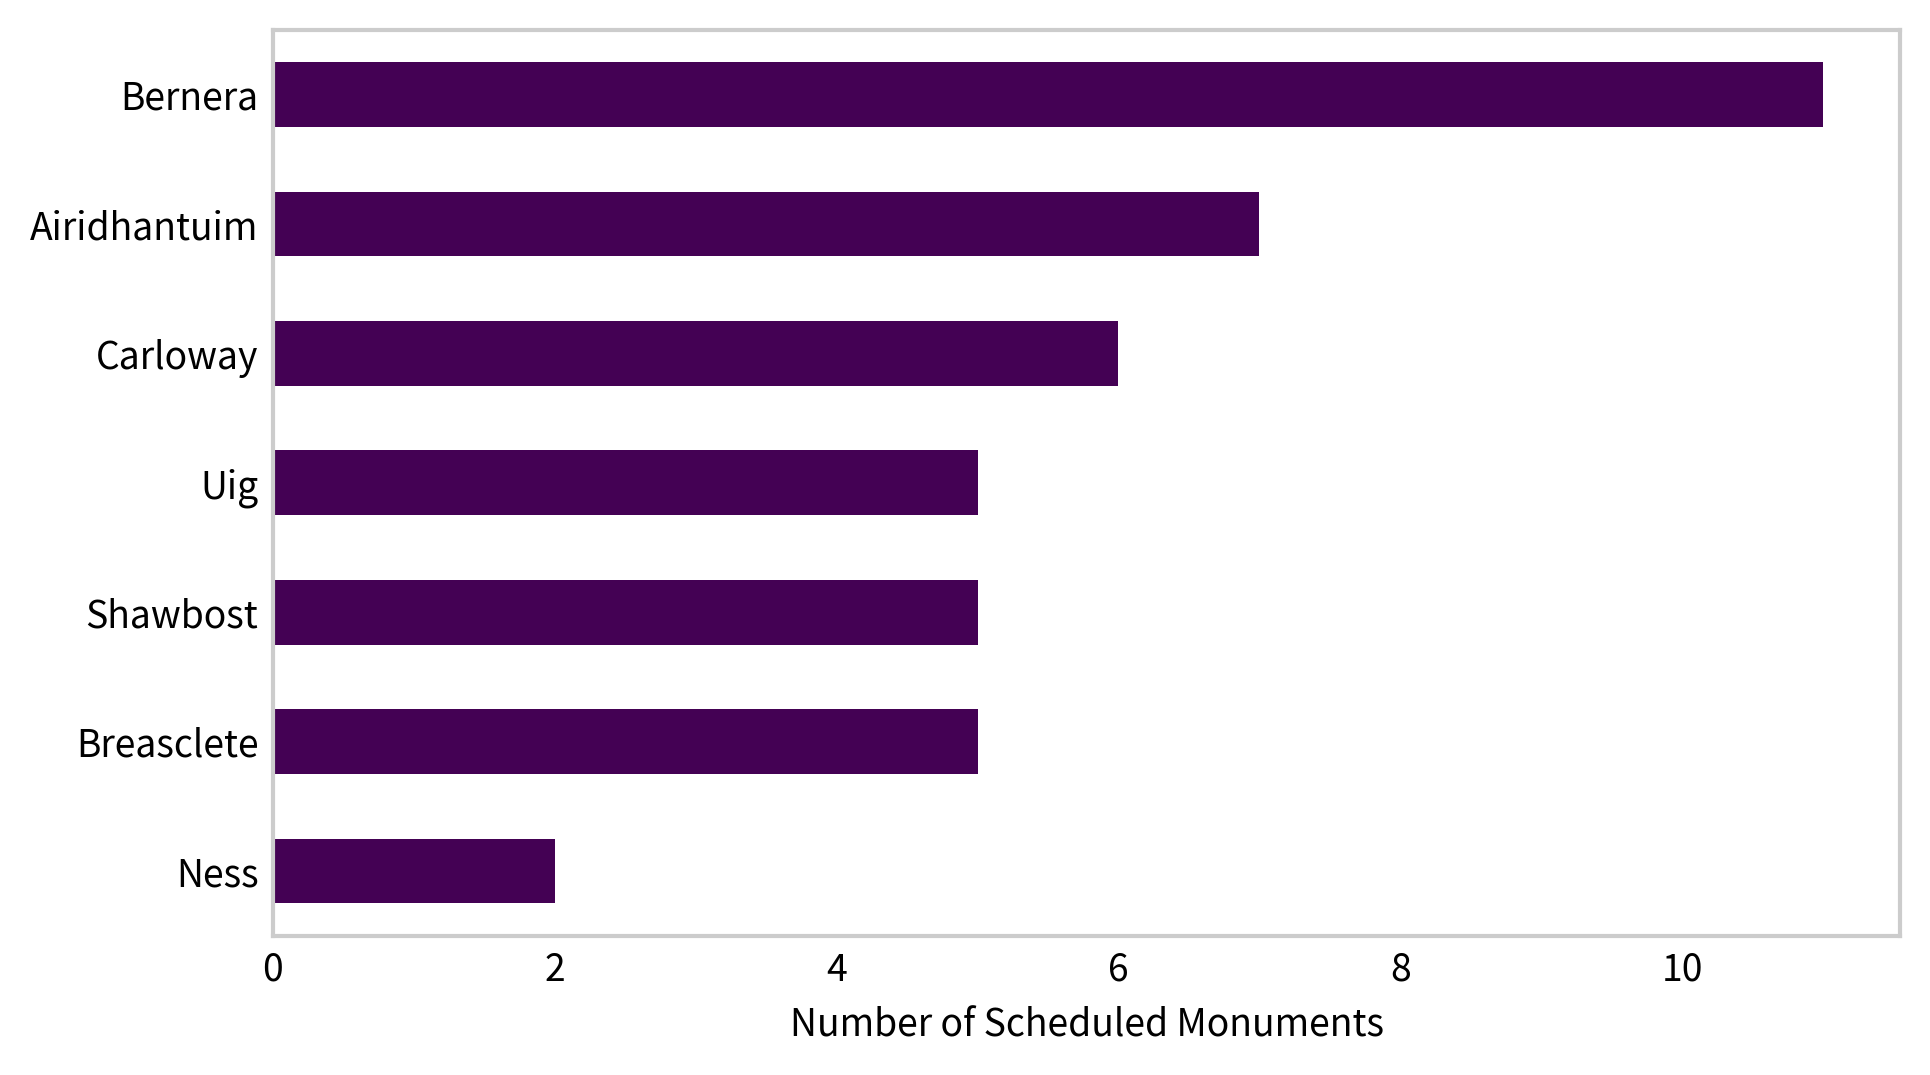
\includegraphics[width=.9\textwidth]{../images/plots/viewpoints_cc}}
  \caption{A chart summarising the number of scheduled monuments in each community council intersecting the study area. \label{fig:sm-cc}}
\end{figure}

The final viewpoints were selected based on the prevalence of photographic data available on Wikimedia Commons and Geograph \autocite{wikimedia,geograph-uk} (which indicates the popularity of certain sites), as well as some inputs from community land owners during the participatory \gls{gis} session. These viewpoints were filtered from the scheduled monuments data using Python. The distribution of the viewpoints is shown in \autoref{fig:vp-loc}, while photographs of viewpoints can be seen in \autoref{fig:viewpoints1} and \autoref{fig:viewpoints2}.

\begin{figure}
  \centering
  \includegraphics{../images/maps/viewpoints}
  \caption{A map showing the location of viewpoints in each community council that intersects the study area. \label{fig:vp-loc}}
\end{figure}

\begin{figure}
  \centering
  \begin{subfigure}[t]{.48\textwidth}
    \frame{\includegraphics[width=\textwidth]{../images/viewpoints/Calanais_Standing_Stones}}
    \caption*{Callanish Standing Stones, Breascelte (121301, 932992), SM90054. Photo: CC-BY-SA-3.0 - \textcopyright~Otter - Wikimedia Commons. 10 June 2009. \url{https://commons.wikimedia.org/wiki/File:Calanais_Standing_Stones_20090610_01.jpg}.}
  \end{subfigure}
  ~
  \begin{subfigure}[t]{.48\textwidth}
    \frame{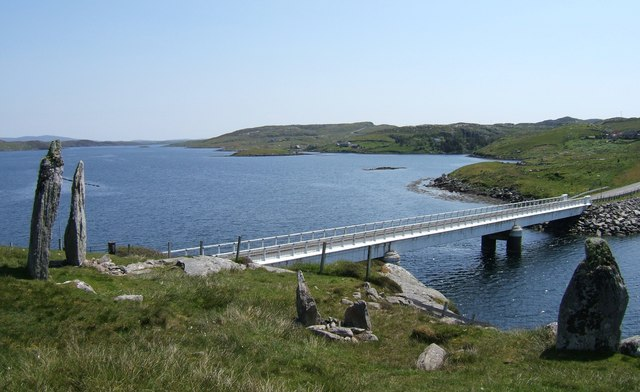
\includegraphics[width=\textwidth]{../images/viewpoints/Bernera_Bridge}}
    \caption*{Bernera Bridge stone setting, Bernera (116385, 934255), SM5548. Photo: CC-BY-SA-2.0 - \textcopyright~F. Leask - Geograph. 8 June 2007. \url{https://www.geograph.org.uk/photo/602195}.}
  \end{subfigure}
  \\[.5cm]
  \begin{subfigure}[t]{.48\textwidth}
    \frame{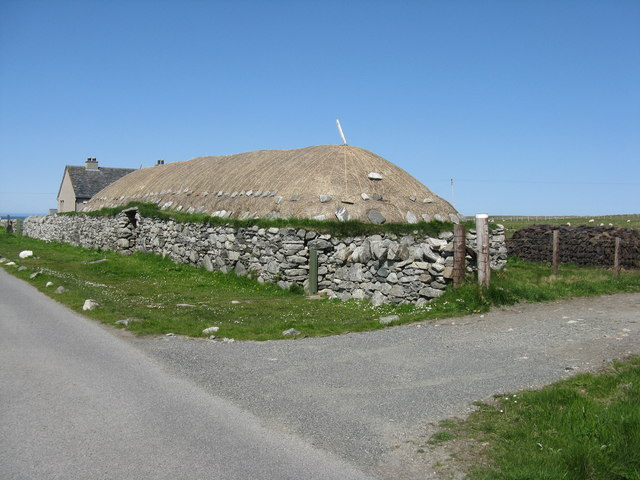
\includegraphics[width=\textwidth]{../images/viewpoints/Arnol_Blackhouse}}
    \caption*{Arnol Blackhouse and associated croft houses, Shawbost (131057, 949253), SM90022. Photo: CC-BY-SA-2.0 - \textcopyright~M J Richardson - Geograph. 27 May 2016. \url{https://www.geograph.org.uk/photo/4988136}.}
  \end{subfigure}
  ~
  \begin{subfigure}[t]{.48\textwidth}
    \frame{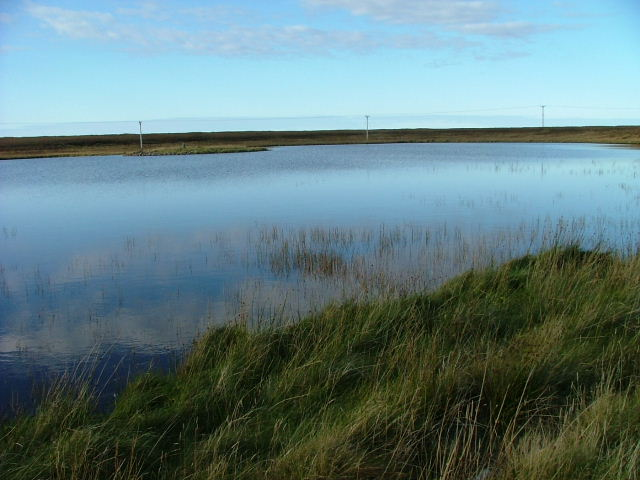
\includegraphics[width=\textwidth]{../images/viewpoints/Loch_Barabhat}}
    \caption*{Loch Baravat dun, North Galson, Ness (146172, 959665), SM5454. Photo: CC-BY-SA-2.0 - \textcopyright~Dave Fergusson - Geograph. 29 September 2007. \url{https://www.geograph.org.uk/photo/573109}.}
  \end{subfigure}
  \caption{Photographs of viewpoints in Breascelte, Bernera, Shawbost, and Ness within the study area. All viewpoints are designated scheduled monuments. \label{fig:viewpoints1}}
\end{figure}

\begin{figure}
  \centering
  \begin{subfigure}[t]{.48\textwidth}
    \frame{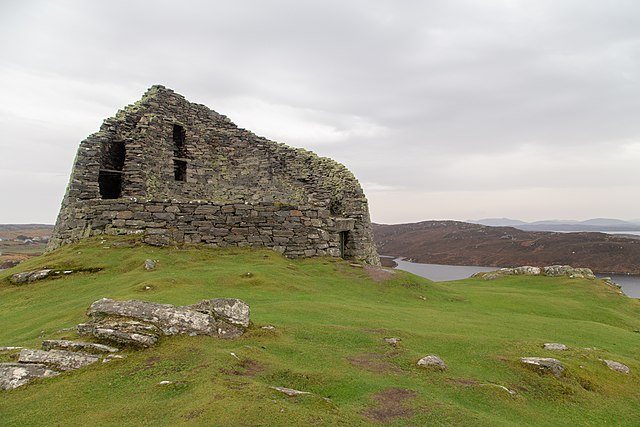
\includegraphics[width=\textwidth]{../images/viewpoints/Dun_Carloway}}
    \caption*{Dun Carloway broch, Carloway (119002, 941231), SM90110. Photo: CC-BY-SA-2.0 - \textcopyright~Tom Parnell - Flickr/Wikimedia Commons. 25 February 2019. \url{https://commons.wikimedia.org/wiki/File:Dùn_Chàrlabhaigh_(40814409303).jpg}.}
  \end{subfigure}
  ~
  \begin{subfigure}[t]{.48\textwidth}
    \frame{\includegraphics[width=\textwidth]{../images/viewpoints/Steinacleit}}
    \caption*{Steinacleit homestead and field system, Airidhantuim (139652, 954086), SM90284. Photo: CC-BY-SA-4.0 - \textcopyright~Andrew Gray - Wikimedia Commons. 11 April 2018. \url{https://commons.wikimedia.org/wiki/File:Outer_Hebrides_-_Steinacleit_-_20180411114215.jpg}.}
  \end{subfigure}
  \\[.5cm]
  \begin{subfigure}[t]{.48\textwidth}
    \frame{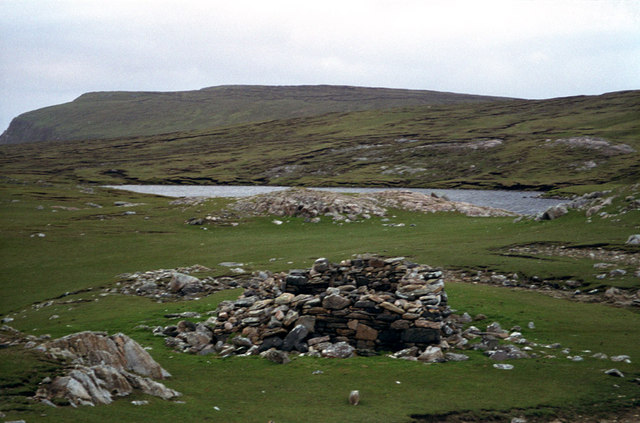
\includegraphics[width=\textwidth]{../images/viewpoints/Taigh_a_Bheannaich}}
    \caption*{Tigh a' Bheannaich chapel, Uig (103870, 937914), SM5390. Photo: CC-BY-SA-2.0 - \textcopyright~Marc Calhoun - Geograph. 31 May 2001. \url{https://www.geograph.org.uk/photo/683286}.}
  \end{subfigure}
  \caption{Photographs of viewpoints in Carloway, Airidhantuim, and Uig within the study area. All viewpoints are designated scheduled monuments. \label{fig:viewpoints2}}
\end{figure}

The scheduled monuments data were polygon features, so the viewpoints must be converted to point features. This was done using QGIS's centroid algorithm. To calculate zonal statistics for each viewpoint, a buffer of 100 m was applied to each point. Finally, zonal statistics for each scenario at the viewpoints were calculated by iterating over the six normalised viewshed rasters and applying QGIS's zonal statistics algorithm. The statistics calculated are minimum, maximum, mean, and standard deviation.

\clearpage
\section{Site suitability assessment}

\gls{mca} was used to evaluate the suitability of the area within site N4 for commercial-scale offshore wind development. The suitability is analysed in terms of impacts on the community; the lower the impact, the higher the suitability. Based on the review of recent literature \autocite{gaveriaux2019,mekonnen2015,vasileiou2017,tercan2020,deveci2020,mahdy2018,basset2021}, two categories of community impact assessment criteria were identified: socio-economic, such as population and recreational activities; and environmental, such as marine habitats and scenic views. As the focus is on community impacts, site N4's suitability in terms of geology, meteorology, and other natural conditions are omitted from this analysis.

The proximity to the shoreline, scenic areas, and populated areas are factors that influence visual and noise impacts. Meanwhile, installation of offshore turbines must be prohibited where marine species are present, as this is a constraint.

A visual representation of the criteria used is shown in \autoref{fig:criteria}.

\begin{figure}
  \centering
  \includegraphics{../images/maps/criteria}
  \caption{A map showing the locations of census centroids, species distribution, and National Scenic Areas relative to site N4. These are used as criteria, in addition to the coastline, in the MCA study. \label{fig:criteria}}
\end{figure}

Using QGIS, the OS Terrain 50 land-water boundary lines which use the mean low water levels were used as the shoreline. The National Scenic Areas dataset, which comprises of polygons, was used to represent the scenic areas. The multi-ring buffer algorithm was then used to calculate the proximity to scenic areas and the shoreline, using 5 km buffer intervals, which is based on the 3-mile value used by \textcite{mekonnen2015}. The generated buffers were then rasterised to GeoTIFF files of the same resolution as the \gls{dtm}. The population data was based on Scotland's 2011 census output areas and their population-weighted centroids. Heatmaps were used to interpolate the population data from the centroids, which also produces a raster layer.

After clipping the rasters to the study area, they were normalised to a scale of 0 to 1. The normalised rasters were then reclassified into five discrete classes, which represent "very high", "high", "medium", "low", and "very low". The higher the distances to shore and scenic areas, the lower the anticipated impacts on the community; therefore, the higher the suitability for offshore development. Conversely, the higher the interpolated population value, the higher the anticipated impacts on the community; therefore, the lower the suitability for offshore development.

The reclassified raster layers were then added to produce a cumulative raster through the use of the raster calculator. Finally, buffers were created around marine species distribution points, which were weighted by their species count attributes. 1 km exclusion zones were then created to remove these constraints from the site suitability analysis.

\section{Participatory GIS}

A participatory \gls{gis} session was held to solicit local knowledge and opinions from a number of land owners within the study area who will be affected by offshore wind development at site N4. This was an online meeting for two hours done in a General Data Protection Regulation (GDPR) compliant manner using the University of Aberdeen-provided Microsoft Teams account. As a supplementary visual aid, a web map created using ArcGIS Online, containing layers of cultural, natural, and marine features in the study area, was presented to them. The local knowledge obtained through this session is used to complement and adjust inputs used for the visual impact assessment and \gls{mca}, such as viewpoint selection.

An initial consultation took place with a representative of the land owners to survey the number of participants interested, as well as whether there are any special accessibility requirements for the session. This survey was used to develop a full ethical review, which was then submitted to the university for approval. The university data protection office was also contacted for advice. Once approval was granted, the land owners were contacted and the meeting was arranged.

In line with the university's recommendations, the session was planned to be recorded using Microsoft Teams, which was then transcribed into qualitative data. The participants were informed of this beforehand, as well as notified that their participation is voluntary and that they may withdraw at any point. Once the necessary data was transcribed, the recording was securely deleted to minimise risks and protect the privacy of the participants.

The questions listed below formed the basis of the discussion during the participatory session:

\begin{enumerate}[noitemsep]
  \item Which settlement are you based in?
  \item What are the most important economic activities, heritage sites, and scenic views in your settlement and the Isle of Lewis in general?
  \item In your opinion, what are the biggest advantages and disadvantages of developing the N4 site into an offshore wind farm to your settlement and Lewis communities in general? Is there anything that concerns you the most?
  \item Do you think the study area defined in this project is sufficient to capture the impacts on your settlement and community?
  \item Can you rank the offshore wind farm development criteria for the N4 site from most to least important in the context of your settlement as well as Lewis communities in general? Criteria include proximity to heritage sites and protected areas.
  \item Do you believe there are any development criteria that may have been overlooked or are missing from this analysis?
  \item Based on the different development scenarios (in terms of number (density) and height of wind turbines installed), which scenario do you believe is the most appropriate for Lewis communities?
  \item What are the most important viewpoints to various visual receptors in the affected area (i.e. the people in your settlement, Lewis communities in general, and visitors)?
  \item Are there any sites and important scenic viewpoints that you would consider more important than the others? What are the reasons for your choices?
  \item What are the most important landscapes and seascapes in the affected area? Have there been any significant changes to these (both naturally and through human activity) over time?
  \item Do you anticipate any other positive or negative impacts if site N4 was to be developed?
  \item Were you consulted at any point during the development of the Sectoral Marine Plan for Offshore Wind (2020)? If yes, please provide some details on the consultation method, frequency, and information provided.
  \item There is a significant change between the scoping area and final plan option of site N4 published in the Sectoral Marine Plan. What is your opinion on this?
  \item Has there been any other public engagement once the N4 site was proposed? What are your expectations for future engagement?
  \item What was your experience in using the web map provided during this session? Was it easy to use and interpret, and did it help you visualise the affected areas?
  \item Do you have any feedback on how this session can be improved? Additionally, do you believe a participatory GIS framework can be used to improve public engagement in the future?
\end{enumerate}

The land owners were informed that they may provide rankings to indicate the relative importance of factors (e.g. in a scale of 1 to 10, where 1 is least important and 10 is most important). Additionally, they were able to use the web map, which supports anonymous public data collection, to directly indicate locations of interests and optionally add points, lines, and polygons of important locations.

A participant information sheet and consent form was developed and provided to the participants ahead of the meeting. The participant materials can be viewed in \autoref{app:pgis}.
